
\graphicspath{ {\curdir/Graphics/}  }

The two ion species that were chosen to load into these traps as part of our computer architecture were barium and ytterbium.  These elements have several advantages for building a quantum computer using our architecture which will be discussed in this chapter.  Ytterbium will be used to implement the actual quantum computation, while barium will be used to generate remotely entangled ion pairs between ion traps and cool both species.

\section{Ionization}
\label{sec:ionization}

Before any of the trapping technology discussed in the previous section will work we need a source of ions. The atoms to be ionized are generated by heating a small alumina oven tube inside the vacuum chamber.  The oven is loaded with small pieces cut from metallic barium or ytterbium before the chamber is sealed.  It is wrapped with small diameter tungsten wire which is then connected to a vacuum feedthrough.  By running currents between 1-2~A (depending on the length of the wire and its contact with the oven) the oven can be heated to a sufficient temperature to emit a usable flux of the neutral atom.  The flux from the oven is difficult to measure directly, but very reasonable trapping rates of a few ions per minute can be achieved with these currents.  Ionization is accomplished by applying lasers energetic enough to strip the outer electron from the atom, often using intermediate states of the neutral atom to provide isotope selectivity or increase the wavelength of the necessary beams.


\begin{figure}
	\centering
	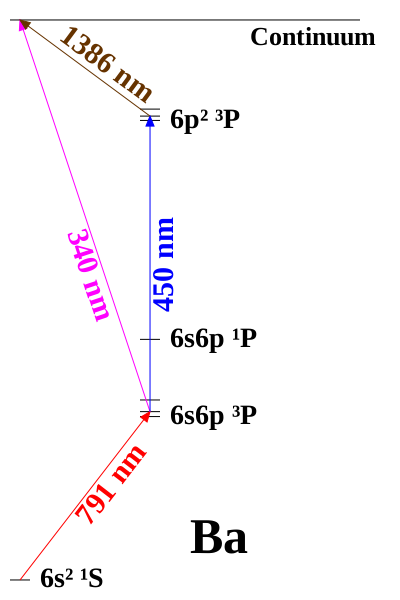
\includegraphics[width=0.5\textwidth]{neutral-Ba}
	\caption[Energy levels of neutral barium]{Energy levels of neutral barium (to scale) \cite{Karlsson:99}.  Possible ionization paths including direct, via 6s6p $^3$P and then direct, and via 6s6p $^3$P and 6p$^2$ $^3$P are shown.}
	\label{fig:neutralba}
\end{figure}

Barium is an alkaline earth metal which makes the atomic structure of its ion easy to analyze.  The spectrum of neutral barium provides many different possibilities for ionization paths as shown in Figure~\ref{fig:neutralba}.  Originally, we directly ionized with a xenon-mercury arc lamp which has ultraviolet spectral components at 237~nm, the ionization threshold of barium.  This method is not isotope selective, and the lamp is generally very difficult to focus.  We then switched to use a two-photon ionization scheme, first driving a transition from the 6s$^2$ $^1$S ground state to a 6s6p $^3$P$_1$ excited state and then ionizing using a 337~nm nitrogen pulse laser.  The first transition, accomplished using a single mode laser diode at approximately 791~nm, provides isotope selectivity.  In addition, both transitions are driven by lasers that can be reasonably well focused near the trapping location.  

The 791~nm laser frequency is stabilized using a side-of-the-fringe locking circuit to a low finesse optical cavity.  This circuit subtracts a constant value from the voltage output of a transimpedance amplifier connected to a photodiode behind the optical cavity.  This voltage provides an error signal that, when fed back to the piezoelectric element in the ECDL with a PID controller, will stabilize the frequency of the laser to a frequency on the side of the cavity line shape.  The cavity itself is temperature stabilized with another PID controller feeding back a temperature signal from a thermistor onto the current through a resistive heater using a MOSFET in the linear regime.  We observe short term frequency stability of a 1-3~MHz and long term drifts of 10-20~MHz, most likely due to residual variation in temperature and changes in atmospheric pressure.

This method of ionization has been very successful for a long time.  The only downside is that it still uses a fairly energetic beam in the 337~nm nitrogen laser.  This laser is energetic enough to easily ionize material deposited on the trap surfaces nearby which can create stray, uncontrolled electric fields that perturb the position of the ion.  This ionization becomes increasingly problematic for wavelengths below 400~nm \cite{Harter:14}.  In macroscopic linear rf traps, this issue has never caused any serious problems because the trap surfaces are several hundred microns from the trapping location and the ionization lasers can be well focused between these surfaces.  When working with surface traps, the trapping region is only separated from the nearest surface by 50-80~microns, and this charging can be a more serious issue.

Therefore, after some initial difficulties trapping in surface traps, we switched to a different ionization scheme that uses only longer wavelength lasers.  The initial step is still the transition driven by the 791~nm laser, but then we instead drive a second intermediate transition to the 6p$^2$ $^3$P$_1$ state using a 450~nm ECDL.  From this excited state the 791~nm or any shorter wavelength laser provides sufficient energy to complete the ionization.  We have successfully used this scheme to ionize barium in surface traps and have not observed excessive charging of the surface during several months of repeated exposure.

\begin{figure}
	\centering
	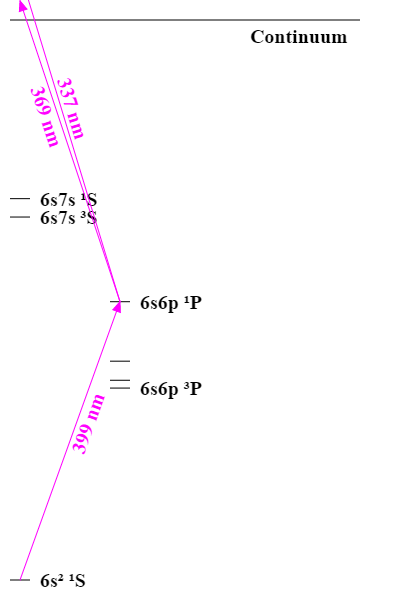
\includegraphics[width=0.5\textwidth]{neutral-Yb}
	\caption[Energy levels of neutral ytterbium]{Energy levels of neutral ytterbiun (to scale) \cite{Sansonetti:05}.  Ionization is achieve using a 399~nm laser and a 369~nm laser.}
	\label{fig:neutralyb}
\end{figure}

Ytterbium is a lanthanoid and has 14 more protons and electrons than barium.  These additional electrons are often bound in the 4f subshell and again, in Yb$^+$ there is a single valence electron in the 6s subshell that is easy to analyze.  There is the additional complication that one of the electrons from the 4f subshell can sometimes be excited to a higher energy subshell giving rise to some additional energy levels with an inner shell vacancy.  Currently we ionize ytterbium using a two-step isotope-selective process.  The neutral atom is addressed with a 399~nm laser that drives a transition from the 6s$^2$ $^1$S ground state to 6s6p $^1$P singlet state which provides isotope selectivity (see Figure~\ref{fig:neutralyb}).  We then ionize using the same nitrogen pulse laser that can be used to ionize barium.  Once we have set up our ytterbium cooling lasers, the 369~nm cooling beam will be a more efficient ionization path from the intermediate state.

\section{Doppler Cooling}
\label{sec:cooling}

When the atoms are ionized they are traveling in a hot thermal beam at a few hundred meters per second, and then suddenly they are affected by the electric fields of the ion trap.  The ions that are trapped need to be cooled to a much lower temperature in order to be well localized so that other operations can be performed on them.  This initial cooling can be accomplished by a technique called laser Doppler cooling.  A strong transition in the ion is addressed by a laser detuned to a frequency slightly lower than the center of the transition.  Cooling is then accomplished using the effect of the Doppler shift because of the ions motion.  When the ion is moving towards the source of the laser, the laser frequency in the ion's rest frame is higher and closer to the center of the resonance.  Therefore the ion absorbs more photons when it is moving towards the laser than when it is moving away from it.  The momentum from these absorptions slows the ion, while the momentum gained from emitting the photons is randomly directed and averages to zero.

The rate at which an ion scatters photons from a laser can be found to be
\begin{equation}
r_{scatter} = \frac{\Gamma}{2} \frac{s}{1 + s + \frac{4 \delta^2}{\Gamma^2}}
\end{equation}
where $\Gamma$ is the linewidth of the atomic transition, $s \equiv \frac{2 \Omega^2}{\Gamma^2}$ is called the saturation parameter, and $\delta$ is the frequency detuning between the source and the center of the atomic transition.  Each photon scattering event also transfers the momentum from the photon to the ions motion.  The resulting force on an ion is
\begin{equation}
	\vec{F}_\mathrm{scatter} = \hbar \vec{k} r_\mathrm{scatter} = \hbar \vec{k} \frac{\Gamma}{2} \frac{s}{1 + s + \frac{4 \delta^2}{\Gamma^2}} \mathrm{.}
\end{equation}
where $\vec{k} = \frac{2 \pi}{\lambda} \hat{k}$ is the photon wavevector.

The Doppler effect modulates this force by causing an additional velocity-dependent frequency shift on the detuning.  The detuning $\delta$ can be rewritten for small ion velocities as $\delta - k v_{ion}$, where $v_{ion}$ is the velocity of the ion with respect to the laser. Cooling can be achieved by choosing these parameters such that the ion experience a force of the form $F = -\gamma v_{ion}$ that acts in opposition to its velocity when $\gamma$ is positive.  For small velocities the force due to photon scattering has the form
\begin{eqnarray}
	F_\mathrm{scatter,doppler} &\approx& F_\mathrm{scatter} - k v_\mathrm{ion} \frac{\partial F_\mathrm{scatter}}{\partial \delta} \\
	&=& F_\mathrm{scatter} \left( 1 + \frac{ 8 k \delta / \Gamma^2 }{ 1 + s + \frac{4 \delta^2}{\Gamma^2} } v_\mathrm{ion} \right)
\end{eqnarray}
where we can identify the term multiplying $v_\mathrm{ion}$ as the damping force coefficient.  For detunings, $\delta$, less than zero this force acts to cool the motion of the ions.

The minimum temperature that can be reached by Doppler cooling is set by the random impulses the ion feels when it emits photons that it has absorbed.  Although these photons are randomly directed and average to no net contribution to the momentum, the ions temperature is still affected by them.  Balancing the cooling rate of the lasers and the heating rate from these random fluctuations, the minimum kinetic energy in the $\hat{x}_i$ direction can be found to be
\begin{equation}
	E_i = \hbar \left( 1 + f_i \frac{r_\mathrm{tot}}{r_\mathrm{i}} \right) \frac{ (\Gamma / 2)^2 + \delta^2 }{8 \delta} \mathrm{,}
	\label{eqn:doppler}
\end{equation}
where $f_i$ is the probability for the ion to scatter a photon in the $\hat{x}_i$ direction and $r_\mathrm{tot}$ and $r_\mathrm{i}$ are the total and fraction due to the beam along the $\hat{x_i}$ direction of the  average scattering rate \cite{Eschner:03, Itano:82}.  We have also assumed that the saturation parameter, $s$, is small.  Figure~\ref{fig:doppler} shows the dependence of the minimum temperature as a function of detuning, $\delta$, for cooling barium ions with a 493~nm laser.  The minimum temperature is $\approx$ 0.25~mK.

\begin{figure}
	\centering
	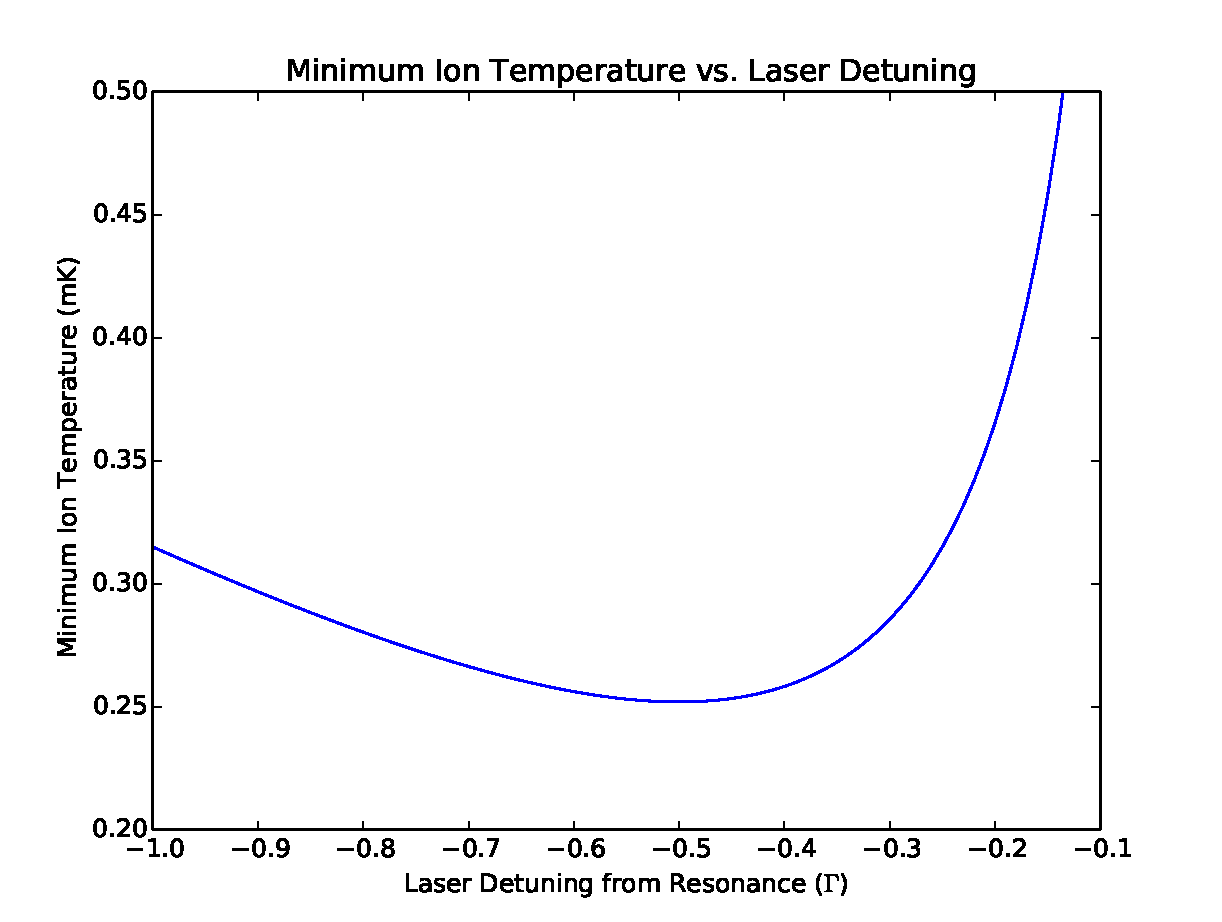
\includegraphics[width=0.8\textwidth]{DopplerCooling}
	\caption[Temperature of Doppler cooled barium ions]{Minimum ion temperature for Doppler cooled barium ions.  The temperature is a function of detuning of the Doppler cooling laser from resonance in units of the natural linewidth $\Gamma$.  The temperature reaches a minimum of $\approx$ 0.25~mK at a detuning of -0.5 $\Gamma$.  Low 493~nm power is assumed and the effect of the 650~nm repump laser is ignored.}
	\label{fig:doppler}
\end{figure}

Doppler cooling barium actually involves using two lasers.  The 493~nm transition scatters the most photons and provides the dominant cooling force.  Unfortunately, there are two possible decay paths from the 6P$_{1/2}$ state that the 493~nm laser excites.  The ion can decay directly back to the 6S$_{1/2}$ ground state from which the 493~nm transition may be driven again to continue cooling, but it may also decay to the long-lived 5D$_{3/2}$ state (see Figure~\ref{fig:ionizedba}).  Since the lifetime of this state is $\approx$ 30~s \cite{Gurell:07} it is necessary to use a second laser to depopulate this state in order to continue to scatter 493~nm photons to cool the ion.  A 650~nm laser is used to drive a transition from the 5D$_{3/2}$ state to the 6P$_{1/2}$ state which closes the cooling cycle because there are no unaddressed decay paths.  This ``repump'' laser complicates the minimum temperature of the ion by introducing an additional laser force as well as two-photon coupling between 6S$_{1/2}$ and 5D$_{3/2}$.  However, when the 650~nm laser is tuned exactly on resonance, the minimum temperature as a function of the 493~nm detuning is only slightly increased.

The 650~nm laser is an external cavity diode laser directly providing approximately 7~mW of optical power, but there were no available 493~nm diodes at the times the setup was designed.  Instead, we have a 986~nm ECDL that produces approximately 150~mW of optical power.  The 986~nm light is sent through an AOM and the first order diffracted beam is sent through a periodically-poled lithium niobate doubling crystal waveguide to produce 493~nm light.  The light can be switched by switching the rf applied to the AOM using a TTL rf switch.  Since this switching is performed in the infrared light, the extinction is squared in the blue light sent to the ion due to the nonlinearity in the frequency doubling process.  We cannot directly measure the actual extinction, but we have determined that it is $>$ 43~dB.  The 650~nm light is shuttered using a single- or double-passed AOM depending on the needs of the experiment being performed (see Figure~\ref{fig:optics}).

\begin{figure}
	\centering
	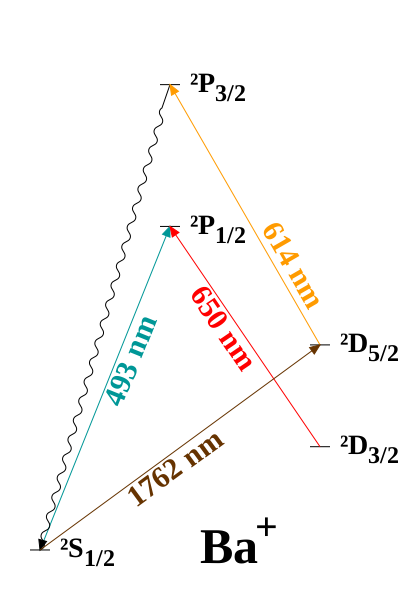
\includegraphics[width=0.5\textwidth]{ionized-Ba}
	\caption[Energy levels of BaII]{Energy levels of singly ionized barium (to scale) \cite{Karlsson:99}.  Laser cooling is accomplished using the 493~nm transition with a 650~nm repump.  The D$_{5/2}$ is used as a ``shelving'' state that is outside of the cooling cycle.  Population can be transferred to D$_{5/2}$ using a 1762~nm laser and returned to the cooling cycle using a 614~nm laser.}
	\label{fig:ionizedba}
\end{figure}

These lasers are already sufficiently stable on short time scales to perform Doppler cooling, but they both exhibit slow frequency drifts on the order of 1~MHz/min that makes it difficult to perform long experiments without stabilization.  For this reason both lasers are stabilized to optical cavities.  The light sent to the optical cavities is offset by an adjustable frequency offset using a DPAOM.  The frequency detuning of the DPAOM is modulated at 20~kHz to modulate the cavity signal.  A phase shifter, frequency mixer, and low pass filter are used to demodulate the cavity signal with the reference 20~kHz modulation signal.  The result is an error signal that crosses zero at the top of the cavity signal.  The error signal is sent through a PID controller and then to a piezoelectric element controlling the feedback frequency inside the ECDL.  As shown in Figure~\ref{fig:optics}, the light being sent to the optical cavity comes from the 0$^{th}$ order of an AOM used for shuttering the light going to the vacuum chamber.  For this reason, the optical power sent to the cavities can vary by a factor of 5 to 10 during an experiment, when the AOMs are frequently turned on and off.  The circuit described here is insensitive to this change in power because it stabilizes the laser to the top of the fringe, whereas the side-of-the-fringe circuit described earlier would cause large frequency shifts whenever the shuttering AOM was switched. 

\begin{figure}
	\centering
	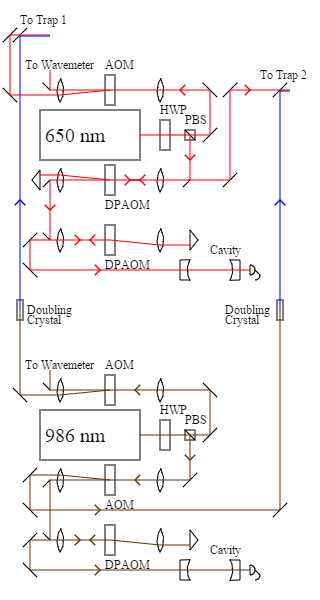
\includegraphics[height=0.6\textheight]{optics-layout}
	\caption[Schematic of optical layout of barium Doppler cooling lasers]{Layout of optics for Doppler cooling barium ions.  A 650~nm ECDL and a 986~nm ECDL are both used. The 986~nm laser is frequency doubled to produce 493~nm light using a nonlinear crystal.  Both lasers are divided into two independent paths to cool ions in two separate vacuum chambers with the amount of power in each beam controllable by a HWP.  The lasers for each trap are then combined using a dichroic mirror and sent to the traps via single mode fiber (not shown).}
	\label{fig:optics}
\end{figure}

A diagram of the Yb$^+$ energy levels is shown in Figure~\ref{fig:ionizedyb}.  The dominant cooling transition is at 369~nm and can be reached using a direct diode.  The $^2$P$_{1/2}$ excited state that is reached via this transition can also decay to a long-lived 5D$_{3/2}$ state.  Unlike in barium, it is most convenient to depopulate this state using a transition to a different excited state formed by exciting an electron from the f shell.  This transition at 935~nm does not introduce any other long-lived possible decay states and the cooling cycle is closed.  There is one other complication in working with ytterbium though.  The ion can be collisionally excited to the 5F$_{7/2}$ state, which has a lifetime of 5.4~years.  We currently do not have any way to repump from this state, which will limit the useful lifetimes of the ytterbium we trap.

The ytterbium lasers are not currently shuttered in any way, although that will be necessary to perform quantum operations on ytterbium ions eventually.  They are again stabilized to optical cavities using a side of the fringe locking circuit similar to the one used with the 791~nm laser.  We are making final preparations to begin using them for cooling the ytterbium ions we have already trapped.

\begin{figure}
	\centering
	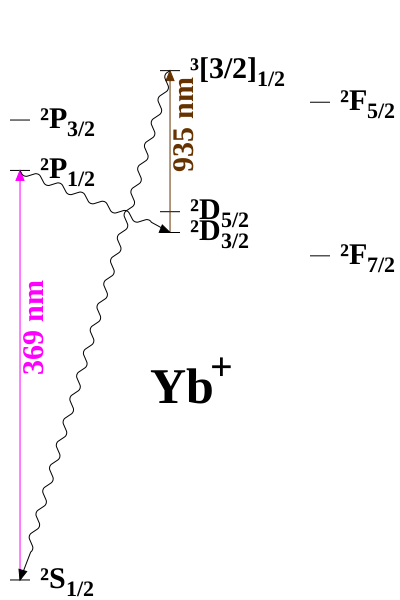
\includegraphics[width=0.5\textwidth]{ionized-Yb}
	\caption[Energy levels of YbII]{Energy levels of singly ionized ytterbium (to scale) \cite{Sansonetti:05}.  Laser cooling is accomplished using the 369~nm transition with a 935~nm repump. The $^2$F$_{7/2}$ state can be collisionally excited and has a lifetime of 5.4~years \cite{Roberts:00}, but can be repumped using a 638~nm laser when this limit to our useful ion lifetime becomes problematic.}
	\label{fig:ionizedyb}
\end{figure}

\section{Initialization and Readout}
\label{sec:initread}

Now we have successfully ionized, trapped, and cooled both barium and ytterbium ions.  In order to begin performing quantum information operations on this system, we need to identify qubits in both that will satisfy the DiVincezo criteria from Subsection~\ref{sec:divincenzo}.  In particular we need to choose two energy states that can be initialized to some simple state representing $\ket{0}$, stay coherent for long enough for our computation to take place, and then be measured.

Ytterbium-171 has some very desirable properties for fulfilling these criteria. It has nuclear spin $\frac{1}{2}$, which means that its 6S$_{1/2}$ ground state is split into two hyperfine levels with $F = 0$ and $F = 1$.  The hyperfine splitting between the two $F$ levels is 12.643~GHZ, and therefore laser line widths are small enough to frequency select which $F$ manifold to address.  The $F = 0$ hyperfine level has only one possible $m_F$ quantum number $m_F = 0$.  The $F = 1$ hyperfine manifold has three levels, $m_F = -1, 0, 1$.  These two $m_F = 0$ levels make excellent qubit levels because they are insensitive to the first order to external magnetic fields.  Coherence times for this qubit of greater than a second have been measured without any kind of magnetic shielding \cite{Olmschenk:07}.  

Initialization and readout of these qubit levels is also very easy.  Readout can be performed by tuning the 369~nm laser to the energy difference between the $F = 1$ manifold in the 6S$_{1/2}$ ground state and the $F = 0$ manifold in the 6P$_{1/2}$ excited state.  Due to angular momentum conservation the decay to the $F = 0$ manifold of the ground state is forbidden.  If the ion was initially in the $F = 1$ qubit level, it will continuously absorb and emit light on this transition until it is off-resonantly driven to the $F = 1$ manifold in the excited state.  Due to the large hyperfine splitting compared to the transition linewidth, thousands of photons can be collected to determine the state with a simple threshold.  Initialization can be performed with a frequency-selective optical pumping scheme.  The 369~nm laser is tuned to the 6S$_{1/2}$ $F = 1$ to 6P$_{1/2}$ $F = 1$ transition because the ion can decay to the unaddressed 6S$_{1/2}$ $F = 0, m_F = 0$ qubit level.  Both of these procedures have been accomplished by applying fixed frequency shifts to the 369~nm laser that can be accomplished by controlling microwaves sent to an EOM for that laser.

Ytterbium-174 has nuclear spin 0 and none of these beneficial properties, but it is more naturally abundant and easier to cool because there are no additional hyperfine levels that need to be addressed to close the cooling cycle.  For this reason, and other experimental limitations we are currently working with Yb-174 instead, but actual quantum computation experiments will use Yb-171 in the future.

Choosing a qubit for operations in barium is somewhat more complicated.  There are three possible isotopes that might be considered for use in quantum computation. Barium-138 is most naturally abundant isotope and it has nuclear spin 0 and therefore no hyperfine structure.  Barium-137 has hyperfine structure because of its nuclear spin I=$\frac{3}{2}$, however this does not give rise to the same nice properties as I=$\frac{1}{2}$.  There are no simple selection rules allowing for easy initialization and detection.  There is an isotope of barium, Ba-133, with nuclear spin I=$\frac{1}{2}$, but it undergoes radioactive decay with a half-life of 10.551~yrs \cite{NuDat}.  Therefore an enriched sample must be used in order to work with this isotope.

Currently we have been working with the easiest isotope, Barium-138. Its ground state is a 6S$_{1/2}$ state with two Zeeman levels $m_J = \pm \frac{1}{2}$.  These levels form a nice qubit, but are very sensitive to magnetic field and maintaining coherence for times longer than $\approx$ 1~ms is quite difficult without magnetic shielding.  Fortunately, following the description of our architecture given earlier, we don't need to store quantum information in this species for long periods of time.  Barium ions can be used to cool the ytterbium ions and to generate remote ion entanglement.  The only time quantum information will be stored in barium is after remote entanglement generation, and this entanglement can easily be transferred to ytterbium ions using a gate sequence of a few hundred microseconds. Since we can work around this short coherence time and the ground state Zeeman levels are otherwise suitable to work with, we have chosen them to be the barium qubit levels in our architecture.  We will still need to be able to initialize and readout these qubit levels in order to perform the remote entanglement and transfer the entanglement to ytterbium ions.

Initialization of these levels is again fairly straightforward.  Circularly polarized light can be utilized to initialize the ion into either Zeeman state.  Because of the conservation of angular momentum, the two circular polarization of light, $\sigma^\pm$, when sent along the quantization axis of the ion, must drive transitions with $\Delta m_J = \pm 1$.  Since the 493~nm transition in ionized barium transfers population between two states with angular momentum $J=\frac{1}{2}$ (see Figure~\ref{fig:ionizedba}), $\sigma^+$ 493~nm light cannot drive a transition from 6S$_{1/2} m_J = +\frac{1}{2}$ to any other state.  However, this light can drive transitions between the 6S$_{1/2}$ $m_J = -\frac{1}{2}$ level and the 6P$_{1/2}$ state. Once the transition is driven, the ion can decay to either ground state Zeeman level.  After the $\sigma^+$ polarized 493~nm light has been applied for a period of time that corresponds to tens of scattering events ($\approx$ 100 $\mu$s), population will accumulate in the $m_J=+\frac{1}{2}$ level because no lasers are addressing this level.

In other trapping systems we have implemented this procedure using two separate 493~nm beams.  One beam is focused onto the ion along the quantization axis with linear polarization and therefore can drive transitions from either Zeeman level and will Doppler cool the ion.  The other beam is sent along the quantization axis with a circular polarization to perform optical pumping.  By shuttering the linearly polarized beam, the ion can be optically pumped to the state the circularly polarized beam does not address.

Since our setup switches the 986~nm beam before it is frequency doubled (see Figure~\ref{fig:optics}) the optical pumping procedure can not be implemented in the same way because we cannot independently shutter two 493~nm beams well.  Instead, a single 493~nm beam is sent to the trap.  The beam passes through a quarter wave plate which initializes it to a circular polarization and then through a Pockels cell.  The Pockels cell is oriented so that when charged to 1.1~kV the 493~nm beam can be rotated back towards linear polarization.  Therefore the 493~nm beam can be switched from performing Doppler cooling to performing optical pumping as quickly as the voltage can be switched in the Pockels cell.  We use a modified piezeoelectric actuator driver circuit to implement this switching in $<$ 2~ms based on a TTL signal.

In order to readout the Zeeman levels of the barium ions we cannot play a simple trick as in ytterbium.  Unfortunately, there are no selection rules to prevent decays from the excited state to either of our qubit states.  Instead we have to transfer the population from one of the qubit states to a long-lived state outside of the cooling cycle.  In Figure~\ref{fig:ionizedba}, we can see that there is such a state, the 5D$_{5/2}$ state.  The 5D$_{5/2}$ state has a lifetime of 30~s, which is more than sufficient since we can determine whether the ion is in the cooling cycle by monitoring its fluorescence for $<$ 20~ms.

Population can be transferred to the \ba 5D$_{5/2}$ using a narrow, 1762~nm fiber laser.  This laser produces $\approx 5~mW$ of optical power with a linewidth of $\approx 100~Hz$ \cite{Noel:12}.  It is locked to a temperature and pressure stabilized Zerodur optical cavity with a linewidth of 500~kHz \cite{Dietrich:10} with about half of the laser power.  With the power remaining after frequency stabilization, coherent $\pi$-pulses from the 6S$_{1/2}$ ground state to the 5D$_{5/2}$ excited state can be achieved in as short as 10~us.  Since the natural linewidth of the transition and the Rabi frequency with which we drive it are both much smaller than the separation between the two Zeeman levels we can frequency select which Zeeman level we are addressing.  The laser is shuttered by a single pass AOM with a frequency bandwidth of $\approx$ 10~MHz that will also be used to perform frequency scans.

Using this laser readout of the Zeeman state of the \ba ion is achieved by transferring or ``shelving'' one of the Zeeman states to the 5D$_{5/2}$ level.  The cooling lasers are then applied for 20~ms and a simple threshold is used to separate background PMT counts from the counts of a fluorescing ion.  The ion will only be fluorescing if the valence electron was initially in the unshelved Zeeman state.  Once this determination has been made, if the electron was successfully shelved it can be brought back into the cooling cycle without having to wait for the $\approx 30~s$ lifetime by applying light at 614~nm (see Figure~\ref{fig:ionizedba}).

The tools we have developed for manipulating the ground state Zeeman levels of barium will enable us to begin investigating the feasibility of a mixed species ion trap quantum computer.  In Chapter~\ref{sec:modes}, we will analyze the motional modes of these chains and measure their temperatures and heating rates.  In the near future, we will be finishing our development of the infrastructure for working with ytterbium ions.


